\chapter{Introduction}
\label{chap:intro}

\section{Problem Description}

Command line interfaces have been with us since the 1950s
\cite{raymond2004art}. The rise of command line interfaces was closely coupled
with the rise of time-sharing computer systems. Command line interfaces and
time-sharing systems greatly shortened the feedback loop of earlier batch
computing systems and allowed programmers to be able to modify their programs
in near real time. Time-sharing systems also introduced the concept of a
\textit{shell}. A \textit{shell}, a term coined by Louis Pouzin \cite{pouzin},
is a program that allows for interaction with the operating system via textual
commands\cite{mashey1976using}. The \textit{Multics}\cite{corbato1965introduction} operating system
pioneered the concept of operating system shells. The concept proved to be
extremely influential and directly influenced the creation of the
\textit{Thompson shell} for the \textit{UNIX} \cite{ritchie1974unix} operating
system. The \textit{UNIX} shell has arguably had the greatest influence on
command line interfaces as we know them today, as most modern shells are
descendants of the original \textit{UNIX} shell \cite{raymond2004art}.

The command line is still a popular interaction medium for tooling in the areas
of software engineering and system administration
\cite{hultstrand2015git, takayama2006trust}. However, the usage of the command
line in the general personal computing space has practically disappeared
\cite{reimer2005history}. This is especially true for younger individuals,
whose very first exposure to computers has been working with Graphical User
Interfaces (GUIs). This schism in interaction mediums causes issues when the
same younger individuals strive to enter technical fields such as software
development or system administration. The issue is further propagated by the
fact that the command line is its own distinct interaction paradigm based
entirely on writing and reading text. This can mean that the usage of
traditional learning resources such as documentation and manuals might prove
difficult to translate into effective usage without active textual interaction
practice on the part of the learner. On the other hand, jumping straight into
practising on the command line comes with its caveats. The shell can be an
unforgiving tool for a novice user as it is very sensitive to syntax and often
provides feedback that is difficult to understand for novice users. The shell
also interacts directly with the operating system and does not require
confirmation for certain destructive tasks such as file deletion.

\subsection{Solving The Problem} The goal of this Master's thesis is to develop
an interactive learning tool that simultaneously aims to address the previously
introduced issues of lack of exposure to textual interaction, the novice
unfriendly environment of the shell and the difficulties of traditional
learning methodologies. The tool should provide a more forgiving experience
than using the shell directly whilst still being a faithful representation of a
system shell. Concepts learned during the interactive tutorials should be
directly transferrable to a standard Unix-like shell. Furthermore, the tool
should be easy to use and encourage experimentation in order to augment the
learning experience and in order to better exploit the advantages offered by
interactive learning systems.
%TODO: Expand a bit

\subsection{Research Questions}
\label{subsec:rqs}

In this work, we set out to address the following research questions:

\begin{enumerate}[label=\textbf{RQ\arabic*}, leftmargin=*]
	\item Are there identifiable patterns of difficulty when it
	      comes to adopting CLIs? Can the "intimidation factor" be pinned down? \label{rq:1}
	\item How should an interactive learning tool be designed to mitigate
	      the difficulty and intimidation factor of learning CLIs? \label{rq:2}
	\item How can a "forgiving" shell be implemented on top of an existing
	      shell to enable the transition from learning to real-world usage? \label{rq:3}
	\item Is the interactive tool more effective than text-based learning methods? \label{rq:4}
	\item Are novice CLI users more likely to continue
	      using CLI interfaces after using such a tool? \label{rq:5}
\end{enumerate}

\subsection{Why CLIs?}
Before introducing our solution to the stated problem, we would like to discuss
the motivations behind using command line interfaces and lowering the barrier of
entry to their use.

Command line interfaces are still widely employed and being developed for a
variety of uses. Benefitting from their simplicity, Command line interfaces
allow for comparatively rapid development and the implementation of features
when compared to their graphical counterparts, which would require a much more
detailed and complicated implementation and more challenging user interface
considerations. Command line programs also further benefit from simplicity of
their textual nature when it comes to their ability to work with other
programs. The simple notion of textual input and output being the main forms of
interaction allow for an extremely flexible interface\footnote{In this case
	"interface" describes a medium through which programs can communicate, not
	a user interface.} for chaining tools together. This composition of programs is
referred to as \textit{piping} and is a hallmark element of what is considered to be the
\textit{UNIX Philosophy} \cite{mcilroy1978unix}. Since most command line
applications share this philosophy of textual input and output there isn't the
need for bespoke mediums of communication to be developed and features can be
more effectively shared across programs.

Since CLI programs are run within a shell, which has direct access to the
underlying operating system, a tight integration between program and system is
formed. This tight coupling, paired with the low system resource requirements,
the ability to specify inputs and arguments via text and modify program
behaviour upon instantiation with flags opens the room for powerful batch
processing capabilities, easy automation and the ability to deal with large
amounts of input and output efficiently.

Beyond the ease of development and composition, there are user interface
elements of command line interfaces that even influence widely used graphical
tools. Command line interaction features can commonly be found implemented into
the text entry fields of search engines \cite{norman2007breakthrough} and chat
applications. An example of this is the ability to use the up arrow to edit the
previously sent message or the ability to use special syntax, like exclamation
points, to influence search results.

The learning curve of such command line interfaces is however a strong barrier
to widespread adoption and enjoyment of the benefits command line interfaces
may bring. For new users, this learning curve is made steeper by the paradigm
shift in the personal computing space towards graphical user interfaces. In
following section, we will introduce the interactive learning tool,
\textit{CLI-Tutor}, developed as a potential solution that addresses the steep
learning curve of the command line through interactive lessons and a sandboxed
shell environment.


% \fig[0.75\textwidth]{img/vimtutor}{Screenshot of vimtutor}{fig:vimtutor}
\section{Introducing "CLI-Tutor"}
\begin{figure}[htbp]
	\centering
	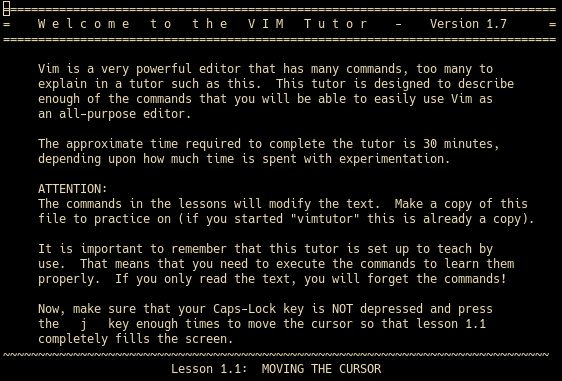
\includegraphics[width=0.75\textwidth]{img/vimtutor}
	\caption{Screenshot of \textit{vimtutor}}
	\label{fig:vimtutor}
\end{figure}

The \textit{CLI-Tutor} tool is an interactive shell-like tutorial program aimed
at making the command line more approachable. We draw inspiration from the
\textit{vimtutor}\cite{pierce_ware_smith_moolenaar_2019} (see: Figure
\ref{fig:vimtutor}) utility shipping alongside the popular terminal-based text
editor \textit{Vim}. \textit{Vimtutor} is an interactive tutorial for the Vim
text editor. It is one long guided lesson presented as a text file. The file
itself contains the basic instructions for editing and creating text within Vim
and is intended to be modified while proceeding through the lesson. This
"learning by doing" approach presented itself as a very suitable approach for
a command line tutorial application. Much like with Vim, where one must learn a new
paradigm of modal editing. When novices learn the command line they are not only
taking on new information about shell usage but also learning an entirely
unfamiliar (textual) interaction paradigm. Newer versions of \textit{vimtutor}
are even more interactive. In the version included in the popular fork of Vim
called \textit{Neovim} \cite{neovimHomeNeovim}, lines intended to be edited by
the user also provide feedback regarding correctness in the form of green
arrows and red crosses.

The \textit{CLI-Tutor} tool introduces users to topics such as shell basics and
Unix-like core utility usage through a series of interactive examples. The tool
aims to relax the steep learning curve associated with the command line by
leveraging interactive examples and a feedback mechanism to instruct and
educate the user about the current stage of the lesson and provide some
feedback based on the inputs of the user. The core of \textit{CLI-Tutor} is
contained within a command line application written in \textit{Go}\footnote{Go
	programming language: \href{https://go.dev/}{https://go.dev/}} and serves as a
standalone application. However, in order to make the learning experience safer
for the user and to encourage exploration, the CLI application has been wrapped
into a web application to form a sandboxed environment that exposes a terminal
over the web. This means the user can use the tutorial application without fear
of causing their own system any harm.

The \textit{CLI-Tutor} application is fully open source and also comes with its
own custom parser and structure for specifying lessons based on
\textit{Markdown}\footnote{A popular plain text markup language.} files.
This means that the material covered by the lessons can be easily contributed
to and distributed, making the tool easily extensible.


\begin{figure}[H]
	\centering
	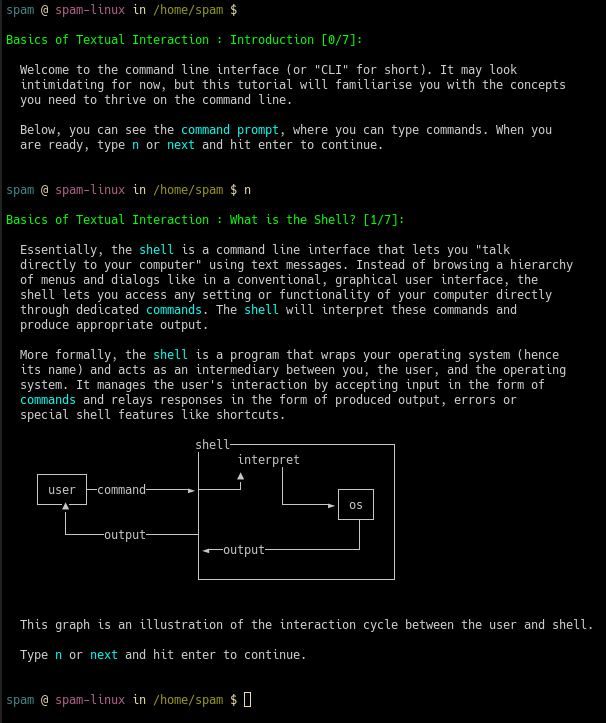
\includegraphics[width=0.75\textwidth]{img/clitutor}
	\caption{Screenshot of \textit{CLI-Tutor}}
	\label{fig:clitutor}
\end{figure}

\section{Thesis Outline}

Over the next few chapters, we will discuss and show the design, implementation
and overall goals of this solution. In \autoref{chap:clitutor}, the semantic
aspects of the \textit{CLI-Tutor} application and associated web application
will be discussed. We will discuss the design and implementation of the
solution in \autoref{chap:design}. \autoref{chap:userstudy}, will discuss the
methodology and introduce the participants of the user study conducted during
this Master's thesis work. Our findings will be discussed in
\autoref{chap:results}. In \autoref{chap:reflection}, we will evaluate and
reflect upon the solution. We will consider existing approaches and make
suggestions regarding building upon and refining \textit{CLI-Tutor}, before,
concluding in \autoref{chap:conclusion}.
